%% arara directives
% arara: xelatex
% arara: bibtex
% arara: xelatex
% arara: xelatex

%\documentclass{article} % One-column default
% \documentclass[twocolumn, switch, 12pt]{article} % Method A for two-column formatting
\documentclass[switch, 12pt]{article}

\usepackage{preprint}

%% Math packages
\usepackage{amsmath, amsthm, amssymb, amsfonts}

%% Bibliography options
\usepackage[numbers,square]{natbib}
\bibliographystyle{unsrtnat}
%\usepackage{natbib}
%\bibliographystyle{Geology}

%% General packages
\usepackage[utf8]{inputenc}	% allow utf-8 input
\usepackage[T1]{fontenc}	% use 8-bit T1 fonts
\usepackage{xcolor}		% colors for hyperlinks
\usepackage[colorlinks = true,
            linkcolor = purple,
            urlcolor  = blue,
            citecolor = cyan,
            anchorcolor = black]{hyperref}	% Color links to references, figures, etc.
\usepackage{booktabs} 		% professional-quality tables
\usepackage{multirow}
\usepackage{nicefrac}		% compact symbols for 1/2, etc.
\usepackage{microtype}		% microtypography
\usepackage{lineno}		% Line numbers
\usepackage{float}			% Allows for figures within multicol
\usepackage{multicol}		% Multiple columns (Method B)
    % \setlength{\columnsep}{0.6cm}

\usepackage[shortlabels]{enumitem}
\setlist[enumerate,1]{leftmargin=2em}

\usepackage{float}
\usepackage{subfloat}
\usepackage{caption}
\usepackage{subcaption}
\usepackage{amssymb}
\usepackage{bbold}
\usepackage{stmaryrd}
\usepackage{graphicx}
\usepackage{tikz}
\usetikzlibrary{bayesnet}
\usetikzlibrary{arrows}
\usepackage{hyperref}

% Section title spacing  options
\usepackage{titlesec}
\titlespacing\section{0pt}{12pt plus 3pt minus 3pt}{1pt plus 1pt minus 1pt}
\titlespacing\subsection{0pt}{10pt plus 3pt minus 3pt}{1pt plus 1pt minus 1pt}
\titlespacing\subsubsection{0pt}{8pt plus 3pt minus 3pt}{1pt plus 1pt minus 1pt}

% Definitions of handy macros can go here
\newcommand{\fracpartial}[2]{\frac{\partial #1}{\partial  #2}}
\newcommand{\prob}{\mathbb{P}} 
\newcommand{\R}{\mathbb{R}}
\newcommand{\N}{\mathbb{N}}
\newcommand{\E}{\mathbb{E}}
\renewcommand{\O}{\mathcal{O}}
\renewcommand{\L}{\mathcal{L}}
\newcommand{\eps}{\varepsilon}
\newcommand{\dd}{\, \mathrm{d}}
\newcommand{\J}{\mathcal{J}}
\DeclareMathOperator*{\argmin}{arg\,min}
\DeclareMathOperator*{\argmax}{arg\,max}
\DeclareMathOperator*{\minimize}{minimize}
\DeclareMathOperator*{\KL}{KL}
\newcommand{\intset}[2]{\{#1, ..., #2\}}
\newcommand{\mnbs}{\nobreak\hspace{.16667em}}
\newcommand{\jump}{\newline\newline}



%%%%%%%%%%%%%%%%   Title   %%%%%%%%%%%%%%%%
\title{Mixture Models for Graph Clustering}

%%%%%%%%%%%%%%%  Author list  %%%%%%%%%%%%%%%
\usepackage{authblk}
\renewcommand*{\Authfont}{\bfseries}
\author[1]{Sofiane Ezzehi}
\author[1]{Bastien Le Chenadec}
\author[1]{Theïlo Terrisse}

\affil[1]{École des Ponts ParisTech}

% Option 2 for author list
%\author{
%  David S.~Hippocampus\thanks{Use footnote for providing further
%    information about author (webpage, alternative
%    address)---\emph{not} for acknowledging funding agencies.} \\
%  Department of Computer Science\\
%  Cranberry-Lemon University\\
%  Pittsburgh, PA 15213 \\
%  \texttt{hippo@cs.cranberry-lemon.edu} \\
%  %% examples of more authors
%   \And
% Elias D.~Striatum \\
%  Department of Electrical Engineering\\
%  Mount-Sheikh University\\
%  Santa Narimana, Levand \\
%  \texttt{stariate@ee.mount-sheikh.edu} \\
%  \AND
%  Coauthor \\
%  Affiliation \\
%  Address \\
%  \texttt{email} \\
%  % etc.
%}

%%%%%%%%%%%%%%    Front matter    %%%%%%%%%%%%%%
\begin{document}

% \twocolumn[ % Method A for two-column formatting
%   \begin{@twocolumnfalse} % Method A for two-column formatting

% \maketitle

% \begin{contribstatement}
%     TODO
% \end{contribstatement}
% %\keywords{First keyword \and Second keyword \and More} % (optional)
% \vspace{0.35cm}

%   \end{@twocolumnfalse} % Method A for two-column formatting
% ] % Method A for two-column formatting

\maketitle

\begin{contribstatement}
    The Daudin-EM was implemented in Numpy and Pytorch by Bastien Le Chenadec. The Newman variant was added by Sofiane Ezzehi, as well as the spectral clustering algorithm. The experiments were performed by Theïlo Terrisse. The report was written by all three authors.
\end{contribstatement}
\vspace{0.35cm}

\begin{multicols}{2}

    \section{Introduction}

    Graph clustering, also referred to as ``community detection'' \cite{fortunato_community_2010}, is the problem of revealing clusters within a graph, where a ``cluster'' is often defined as a set of nodes that are more densely connected between them than with the rest of the network.
    More precisely, a \emph{homophilic} cluster $C$ is defined as a group of nodes with an internal density $\delta_{int}(C)$ larger than its inter-community density $\delta_{ext}(C)$, where
    \begin{equation}
        \delta_{int} = \frac{\text{\# internal edges of }C}{n_C (n_C - 1) / 2}
    \end{equation}
    and
    \begin{equation}
        \delta_{ext} = \frac{\text{\# inter-cluster edges of C}}{n_C (n - n_C)}
    \end{equation}
    with $n$ the number of nodes of the graph, $n_C$ the number of nodes in the cluster $C$.
    % and internal (resp. inter-cluster) edges are edges between nodes of $C$ (resp. between nodes of $C$ and nodes outside of $C$).
    Some applications may also be interested in \emph{heterophilic} clusters, defined such that $\delta_{int}(C) < \delta_{ext}(C)$.
    Graph clustering has tremendous applications in the study of real networks such as
    social [1] or biological [4]. This problem is of importance to perform a mesoscopic study of graphs, where clusters can be interpreted as meta-nodes that reveal new interactions  within a complex system.


    Graph clustering is known to be an NP-hard problem, as testing all possible partitions of a graph has complexity $\O(B_n)$ with $B_n$ the Bell number of order $n$. This is particularly poblematic as real networks easily grow to thousands or even millions of nodes. Several classes of algorithms are documented in the literature \cite{fortunato_community_2010}. To name a few, modularity-based approaches solve an optimization problem that maximizes modularity (defined in Section \ref{subsec:metrics}); hierarchical algorithms rely on similarity measures to aggregate or divide groups of nodes; spectral algorithms also rely on a similarity matrix, but operate in the space spanned by the eigenvectors of its Laplacian matrix. Yet, defining a similiarty measure between nodes is not always trivial.

    Model-based methods are an alternative to algorithmic methods, that aim to fit a mathematical model capable of explaining the observed connectivity, and from which descriptive properties of a graph may be extracted or computed. The Stochastic Block Model (SBM) introduced in \cite{snijders_estimation_1997} is a renowned example of model for graphs. In \cite{main_article}, J.-J. Daudin \textit{et al.} study this model and propose a variational Expectation-Maximization (EM) algorithm to find parameters that best fit a given graph. In this report, their method will be referred to as ``Daudin-EM''.

    In this report, we detail the Daudin-EM method as well as a variant from the literature in Section \ref{sec:method}. In Section \ref{sec:experiments}, we present our implementation of the method and the experiments performed to evaluate it, with a discussion of the results in Section \ref{sec:discussion}. Lastly, we conclude in Section \ref{sec:conclusion}.


    \section{Proposed methods and variants}
    \label{sec:method}

    \subsection{A mixture model for random graphs \cite{main_article}}
    \label{subsec:mixture_model}
    In "A mixture model for random graphs" \cite{main_article}, Daudin \textit{et. al.} propose a bayesian model for graphs, and an EM approach to fit this model to a given graph.

    We will follow the same notations as in \cite{main_article}. We consider an undirected graph with $n$ nodes and no self-loops. We denote $X$ the adjacency matrix of this graph. As such, $X_{ij}\in \{0,1\}$ denotes the existence of an edge between nodes $i$ and $j$, and $\forall i\in \left\{1,\dots,n\right\}, X_{ii}=0$.

    As explained by the authors, the SBM draws inspiration both from mixture models for distribution of degrees, that have the disadvantage of not dealing with the probability for two given nodes to be connected, and from the foundational Erdös-Rényi model, which is known to fit real graphs poorly. To define the SBM, we consider a mixture model that spreads the vertices in $Q$ classes, with an a priori repartition $\{\alpha_1, \dots, \alpha_Q\}$ between classes. We introduce the random variables $Z_{iq} \in \{0,1\}$ for $i\in \left\{1,\dots,n\right\}$ and $q\in \left\{1,\dots,Q\right\}$, that represent the membership of node $i$ to class $q$. We have the following prior distribution on $Z$:
    \begin{equation}
        \forall i\in \left\{1,\dots,n\right\}, \quad \sum_{q=1}^Q Z_{iq} = 1
    \end{equation}
    and
    \begin{equation}
        \label{eq:prior_Z}
        \forall q\in \left\{1,\dots,Q\right\},\quad \mathbb{P}(Z_{iq}=1)=\alpha_q.
    \end{equation}

    We introduce priors on the existence of edges between nodes of different classes. We denote $\pi_{ql}$ the probability of an edge between a node of class $q$ and a node of class $l$. Because the graph is undirected, we have $\pi_{ql}=\pi_{lq}$. This prior writes : $ \forall q,l\in \left\{1,\dots,Q\right\}, \quad \forall i\neq j\in \left\{1,\dots,n\right\},$
    \begin{equation}
        \label{eq:conditional_distribution}
        \mathbb{P}(X_{ij}=1\,|\,Z_{iq}=1,Z_{jl}=1)=\pi_{ql}.
    \end{equation}

    Figure \ref{fig:graphical_model} shows the graphical model of this mixture model.

    \begin{figure}[H]
        \centering
        \tikz{
            \node[obs] (X_{ij}) {$X_{ij}$};
            \node[latent,left=of X_{ij}, xshift=-0.8cm, label={[name=label1,text height=1.2em]below:$i=1,\dots,n$}] (Z_i) {$Z_i$};
            \node[latent,right=of X_{ij}, xshift=0.8cm, label={[name=label2,text height=1.2em]below:$j=i+1,\dots,n$}] (Z_j) {$Z_j$};
            \node[const, above=of X_{ij}](alpha){$\alpha$};
            \node[const, below=of X_{ij}, yshift=-1cm](pi){$\pi$};
            \plate [inner sep=.5cm] {} {(Z_i)(X_{ij})(Z_j)(label1)(label2)} {};
            \plate [inner sep=.25cm] {} {(Z_j)(X_{ij})(label2)} {};
            \edge {Z_i,Z_j} {X_{ij}}
            \edge {alpha} {Z_i}
            \edge {alpha} {Z_j}
            \edge {pi} {X_{ij}}
        }
        \caption{Graphical model of the mixture model}
        \label{fig:graphical_model}
    \end{figure}


    \subsubsection{Variational Expectation-Maximization algorithm}

    The log-likelihood of the model is given by :
    \begin{equation}
        \begin{aligned}
            \log \mathcal{L}(X, Z) = & \sum_{i}\sum_{q} Z_{iq}\log\alpha_q                                                            \\
                                     & + \frac{1}{2}\sum_{i\neq j}\sum_{q,l} Z_{iq}Z_{jl} \, \pi_{ql}^{X_{ij}}(1-\pi_{ql})^{1-X_{ij}}
        \end{aligned}
    \end{equation}

    Because the likelihood $\mathcal{L}(X)$ is not tractable, the authors propose to use an Expectation-Maximization (EM) algorithm to fit the model. However the E-step of the EM algorithm is not tractable either because of the posterior distribution of $Z$ given $X$. Instead the authors propose to optimize $\eqref{eq:lower_bound}$ which is a lower bound of $\log\mathcal{L}(X)$ obtained using the Kullback-Leibler divergence between the posterior distribution of $Z$ given $X$ and an approximated distribution $R_X$.

    \begin{equation}
        \label{eq:lower_bound}
        \mathcal{J}(R_X)=\log \mathcal{L}(X)-\KL[R_X(\cdot), P(\cdot|X)]
    \end{equation}

    By choosing the approximated distribution $R_X$ to be a product of independant multinomial distributions $\eqref{eq:approximated_distribution}$, the authors obtain a fixed point relation $\eqref{eq:fixed_point}$ between the parameters of the model and the parameters of the approximated distribution maximizing the lower bound $\mathcal{J}(R_X)$. This fixed point relation is used in the E-step of the algorithm.
    \begin{equation}
        \label{eq:approximated_distribution}
        \begin{aligned}
            R_X(Z; \tau)=                                 & \prod_{i=1}^n h(Z_i, \tau_i)                     \\
            \forall i \in \left\{1,\dots,n\right\}, \quad & h(Z_i, \tau_i)=\prod_{q=1}^Q \tau_{iq}^{Z_{iq}}.
        \end{aligned}
    \end{equation}
    The fixed point is, $\forall i \in \left\{1,\dots,n\right\}, \forall q \in \left\{1,\dots,Q\right\},$
    \begin{equation}
        \label{eq:fixed_point}
        \hat{\tau}_{iq}\propto \alpha_q \prod_{j\neq i}\prod_l \left[\pi_{ql}^{X_{ij}}(1-\pi_{ql})^{1-X_{ij}}\right]^{\hat{\tau}_{jl}}
    \end{equation}

    This fixed point relation does not assure the theoretical convergence of the algorithm. We will see later that the convergence of the algorithm is not guaranteed in practice either. Finally we have the following updates for the M-step maximizing $\mathcal{J}(R_X)$ :
    \begin{equation}
        \label{eq:m_step}
        \forall q, l \in \left\{1,\dots,Q\right\}, \quad
        \hat{\alpha}_q=\frac{1}{n}\sum_{i} \hat{\tau}_{iq}
    \end{equation}
    and
    \begin{equation}
        \hat{\pi}_{ql}=\frac{\sum_{i\neq j} \hat{\tau}_{iq}\hat{\tau}_{jl}X_{ij}}{\sum_{i\neq j} \hat{\tau}_{iq}\hat{\tau}_{jl}}.
    \end{equation}

    \subsubsection{Selection of $Q$}

    In practice the number of clusters $Q$ has to be estimated. The authors propose to use a criterion based on the Integrated Classification Likelihood (ICL) which writes :
    \begin{equation}
        \begin{aligned}
            \mathrm{ICL}(X, Q) & =\max_\theta\log \mathcal{L}(X, Z \ |\ \theta, Q)-\frac{Q-1}{2}\log n \\&-\frac{1}{2}\times\frac{Q(Q+1)}{2}\log\frac{n(n-1)}{2}
        \end{aligned}
    \end{equation}

    This criterion requires the knowledge of the parameters $\theta$ of the model. We will need to estimate them using the EM algorithm.

    \subsection{An alternative mixture-model by Newman et. al. \cite{newman}}
    \label{subsec:newman}

    A different mixture model has been proposed the same year as Daudin-EM, by Newman \textit{et al.} \cite{newman}. The main difference lies in the way a cluster is defined. In the previous model, the probability of connection between a node in cluster $A$ and a node in cluster $B$ is the same, regardless of the considered nodes.
    \newline
    \newline
    In the Newman model, we build directed edges between nodes. In the undirected case, we simply consider that two nodes are connected if there are directed edges between them in both directions. By construction, $2$ nodes belong to the same cluster if the probability of a directed edge between either of them and any other node in the graph is the same. Therefore, for any given pair of nodes $(i, j)$ belonging to the same cluster $C$ and any other node $k$, we have,
    \begin{equation}
        \mathbb{P}(i \rightarrow k) = \mathbb{P}(j \rightarrow k) = \Pi_{C, k}.
    \end{equation}
    Therefore, we see that matrix $\Pi$, which is different from the $\pi$ of the previous model, describes the probability of a directed edge existing between a cluster and a node. Furthermore, contrary to the previous model, the probability of a directed edge existing between a node in cluster $A$ and a node in cluster $B$ is not necessarily invariant with respect to the considered nodes.

    \subsubsection{Model}

    As in the previous model, we denote $X$ the adjacency matrix of the input graph which is assumed to be undirected and containing $n$ nodes. We also denote $(\alpha_1, \ldots, \alpha_Q)$ the probabilities for a node of belonging to a cluster $q \in \intset{1}{Q}$. We introduce the random variables $g_{i \in \intset{1}{n}} \in \intset{1}{Q}$ which represent the cluster of node $i$; these are analogous to the random variables $Z_{iq}$ previously introduced. Therefore,
    \begin{equation}
        \forall i \in \intset{1}{n}, \quad \mathbb{P}(g_i = q) = \alpha_q.
    \end{equation}
    Finally, we introduce the matrix $\Pi \in [0, 1]^{Q \times n}$ defined earlier.
    Since the input graph is undirected,
    % we consider that an undirected edge exists between two nodes if there are directed edges between them in both directions. Therefore,
    the probability of an undirected edge existing between two nodes $i$ and $j$ is,
    \begin{equation}
        \mathbb{P}(X_{ij} = 1) = \mathbb{P}(i \rightarrow j) \mathbb{P}(j \rightarrow i) = \Pi_{g_i, j} \Pi_{g_j, i}.
    \end{equation}
    Two normalization conditions are imposed,
    \begin{equation}
        \sum_{q = 1}^Q \alpha_q = 1 \quad \text{ and } \quad \forall q \in \intset{1}{Q}, \sum_{i = 1}^n \Pi_{q, i} = 1
    \end{equation}
    \subsubsection{Expectation-Maximization algorithm}

    The expected log-likelihood (with respect to the random variables $g$) is,
    \begin{equation}
        \mathcal{L}(X) = \sum_{i=1}^n\sum_{q=1}^Q \tau_{iq} \left[ \log(\alpha_q) + \sum_{j=1}^n X_{ij} \log(\Pi_{q, j}) \right]
    \end{equation}
    where $\tau_{iq} = \mathbb{P}(g_i = q | X, \alpha, \Pi)$.
    \newline
    \textbf{Remark} : The authors of the article made the surprising choice of not taking into account, in the likelihood of $X$ given the parameters, the probability of the non-existing edges. Taking them into account would have added in the last sum of the log-likelihood a term of the form $(1 - X_{ij}) \log(1 - \Pi_{q, j})$.
    %add colored text
    \jump
    The main advantage of this model is that the expectation step is much simpler than in the previous model as it doesn't require to solve a fixed-point problem. Indeed, we have an explicit expression for $\tau_{iq}$,
    $$ \tau_{iq} = \frac{\alpha_q\prod_{j=1}^N \Pi_{qj}^{X_{ij}}}{\sum_{s=1}^Q \alpha_s\prod_{j=1}^N \Pi_{sj}^{X_{ij}}}.$$
    The M-step updates are,
    $$ \alpha_q = \frac{1}{n} \sum_{i=1}^n \tau_{iq} \quad\text{ and }\quad \Pi_{qj} = \frac{\sum_{i=1}^n X_{ij}\tau_{iq} }{\sum_{i=1}^n k_i \tau_{iq}}.$$
    where $k_i = \sum_{j=1}^n X_{ij}$ is the degree of node $i$. We verify that the normalization conditions are satisfied.

    \subsection{Spectral clustering}
    \label{subsec:spectral}
    A third method that we will use as a comparison baseline is spectral clustering, first introduced in \cite{spectral}. The idea is to use the eigenvectors of the Laplacian matrix of the graph to cluster the nodes. The Laplacian matrix is defined as $ L = D - X$ where $X$ is the adjacency matrix of the graph and $D$ is the diagonal matrix of degrees of the nodes.
    \jump
    The algorithm is simple: stacking the $k$ first eigenvectors of $L$ in a matrix $U \in \mathbb{R}^{n \times k}$, we perform a $k$-means clustering on the rows of $U$.

    \section{Experiments}
    \label{sec:experiments}

    The experiments we have carried out can be separated into three parts, all based on a re-implementation the methods covered in Section \ref{sec:method}. A first experiment illustrates the lack of robustness of the fixed-point algorithm used in the E-step of the Daudin-EM algorithm.
    Second, Daudin-EM is tested isolately on synthetic graphs generated from the SBM introduced in Section \ref{subsec:mixture_model}. This set of experiments aims at studying the capacity of the proposed variational EM algorithm to recover parameters for given graphs, but also the efficiency of the model in terms of graph clustering.
    Lastly, the performance of the mixture model is evaluated on classical real datasets, namely Zachary's Karate club and the Cora dataset. This performance is compared to the baselines presented in Sections \ref{subsec:newman} and \ref{subsec:spectral}.

    \subsection{Implementation}

    All of the experiments were performed using the code attached with this report. The Daudin-EM method (simply referred to as ``SBM'' in the code) was implemented in Python using Numpy, and later in Pytorch to distribute the computations on a GPU. A second Pytorch implementation was added to handle memory issues occurring for large graphs. The Newman variant was directly implemented in Pytorch. As an indication, a speed comparison \textcolor{red}{Est-elle à jour ?} between the versions of the mixture model is available in appendix \ref{app:speed_comparison}. The spectral clustering algorithm was implemented in Numpy in a dedicated notebook. Lastly, the algorithm proposed by Lancichinetti, Fortunato, and Kertesz in \cite{lancichinetti_detecting_2009} to deal with overlapping communities was implemented in Numpy, but was not exploited in experiments for conciseness of this report. %due to a lack of time and to avoid exploring too many directions

    The implementation also comes with a battery of tests to validate the implementations, as well as scripts and notebooks to reproduce and visualize the experiments. All experiences used Pytorch implementations when available, especially the \texttt{PytorchLogImplementation} for Daudin-EM, except for the smallest graphs of the second set of experiments that used the Numpy version as it was faster in this case. For visualizations, we used the Networkx library.

    \subsection{Robustness of the fixed-point algorithm}
    \label{subsec:robustness}

    Early stages of the implementation of the method revealed a lack of robustness of the fixed-point algorithm used in the E-step of the method. In particular, the fixed-point algorithm was found to be sensitive to the initialization of the parameters $\alpha$ and $\pi$, and does not converge in all cases.

    To illustrate this, we perform 2 experiments:
    \begin{enumerate}
        \item In the first experiment, we initialize $50$ random graphs and fix a random $\hat{\tau}$ to get $50$ initial states.
        \item In the second experiment, we fix a random graph and initialize $50$ random $\hat{\tau}$ to get $50$ initial states.
    \end{enumerate}
    In each experiment, the graphs are generated using the SBM described in Section \ref{subsec:mixture_model}, with $Q=3$ and $100$ nodes. More precisely, $\alpha$ and $\pi$ are initialized randomly, then the latent variable $Z$ is sampled from \eqref{eq:prior_Z}, and finally the adjacency matrix $X$ is sampled from \eqref{eq:conditional_distribution}. Random $\hat{\tau}$s are sampled as a normalized uniform variable.
    % To generate a random graph, we first sample $\pi$ by sampling $U \sim \mathcal{U}([0, 1))$, defining $\pi = U U^T$ and normalizing the rows of $\pi$. Each row is also multiplied by $\frac{1}{2}$ to set the density of the connectivity of the graph. Then, we sample $\alpha$ from a Dirichlet law of variable $1.5$. Later, the latent variable $Z$ is sampled from \eqref{eq:prior_Z} and the adjacency matrix $X$ is sampled from \eqref{eq:conditional_distribution}. A random $\hat{\tau}$ is sampled as a normalized uniform variable.
    In each experiment, $100$ fixed-point algorithm iterations are run. These fixed-point iterations are run in parallel for the $50$ initial states, resulting in figures \ref{fig:fixed_point_cv_tau} and \ref{fig:fixed_point_cv_X} which plot the norm of the difference of $\hat{\tau}$ between two successive iterations as a function of the iteration, for all graphs, and for the two experiences.

    Code for this experiment is available in file \texttt{fixed\_point\_convergence.py}.


    \begin{figure*}
        \centering
        \begin{subfigure}{0.49\linewidth}
            \centering
            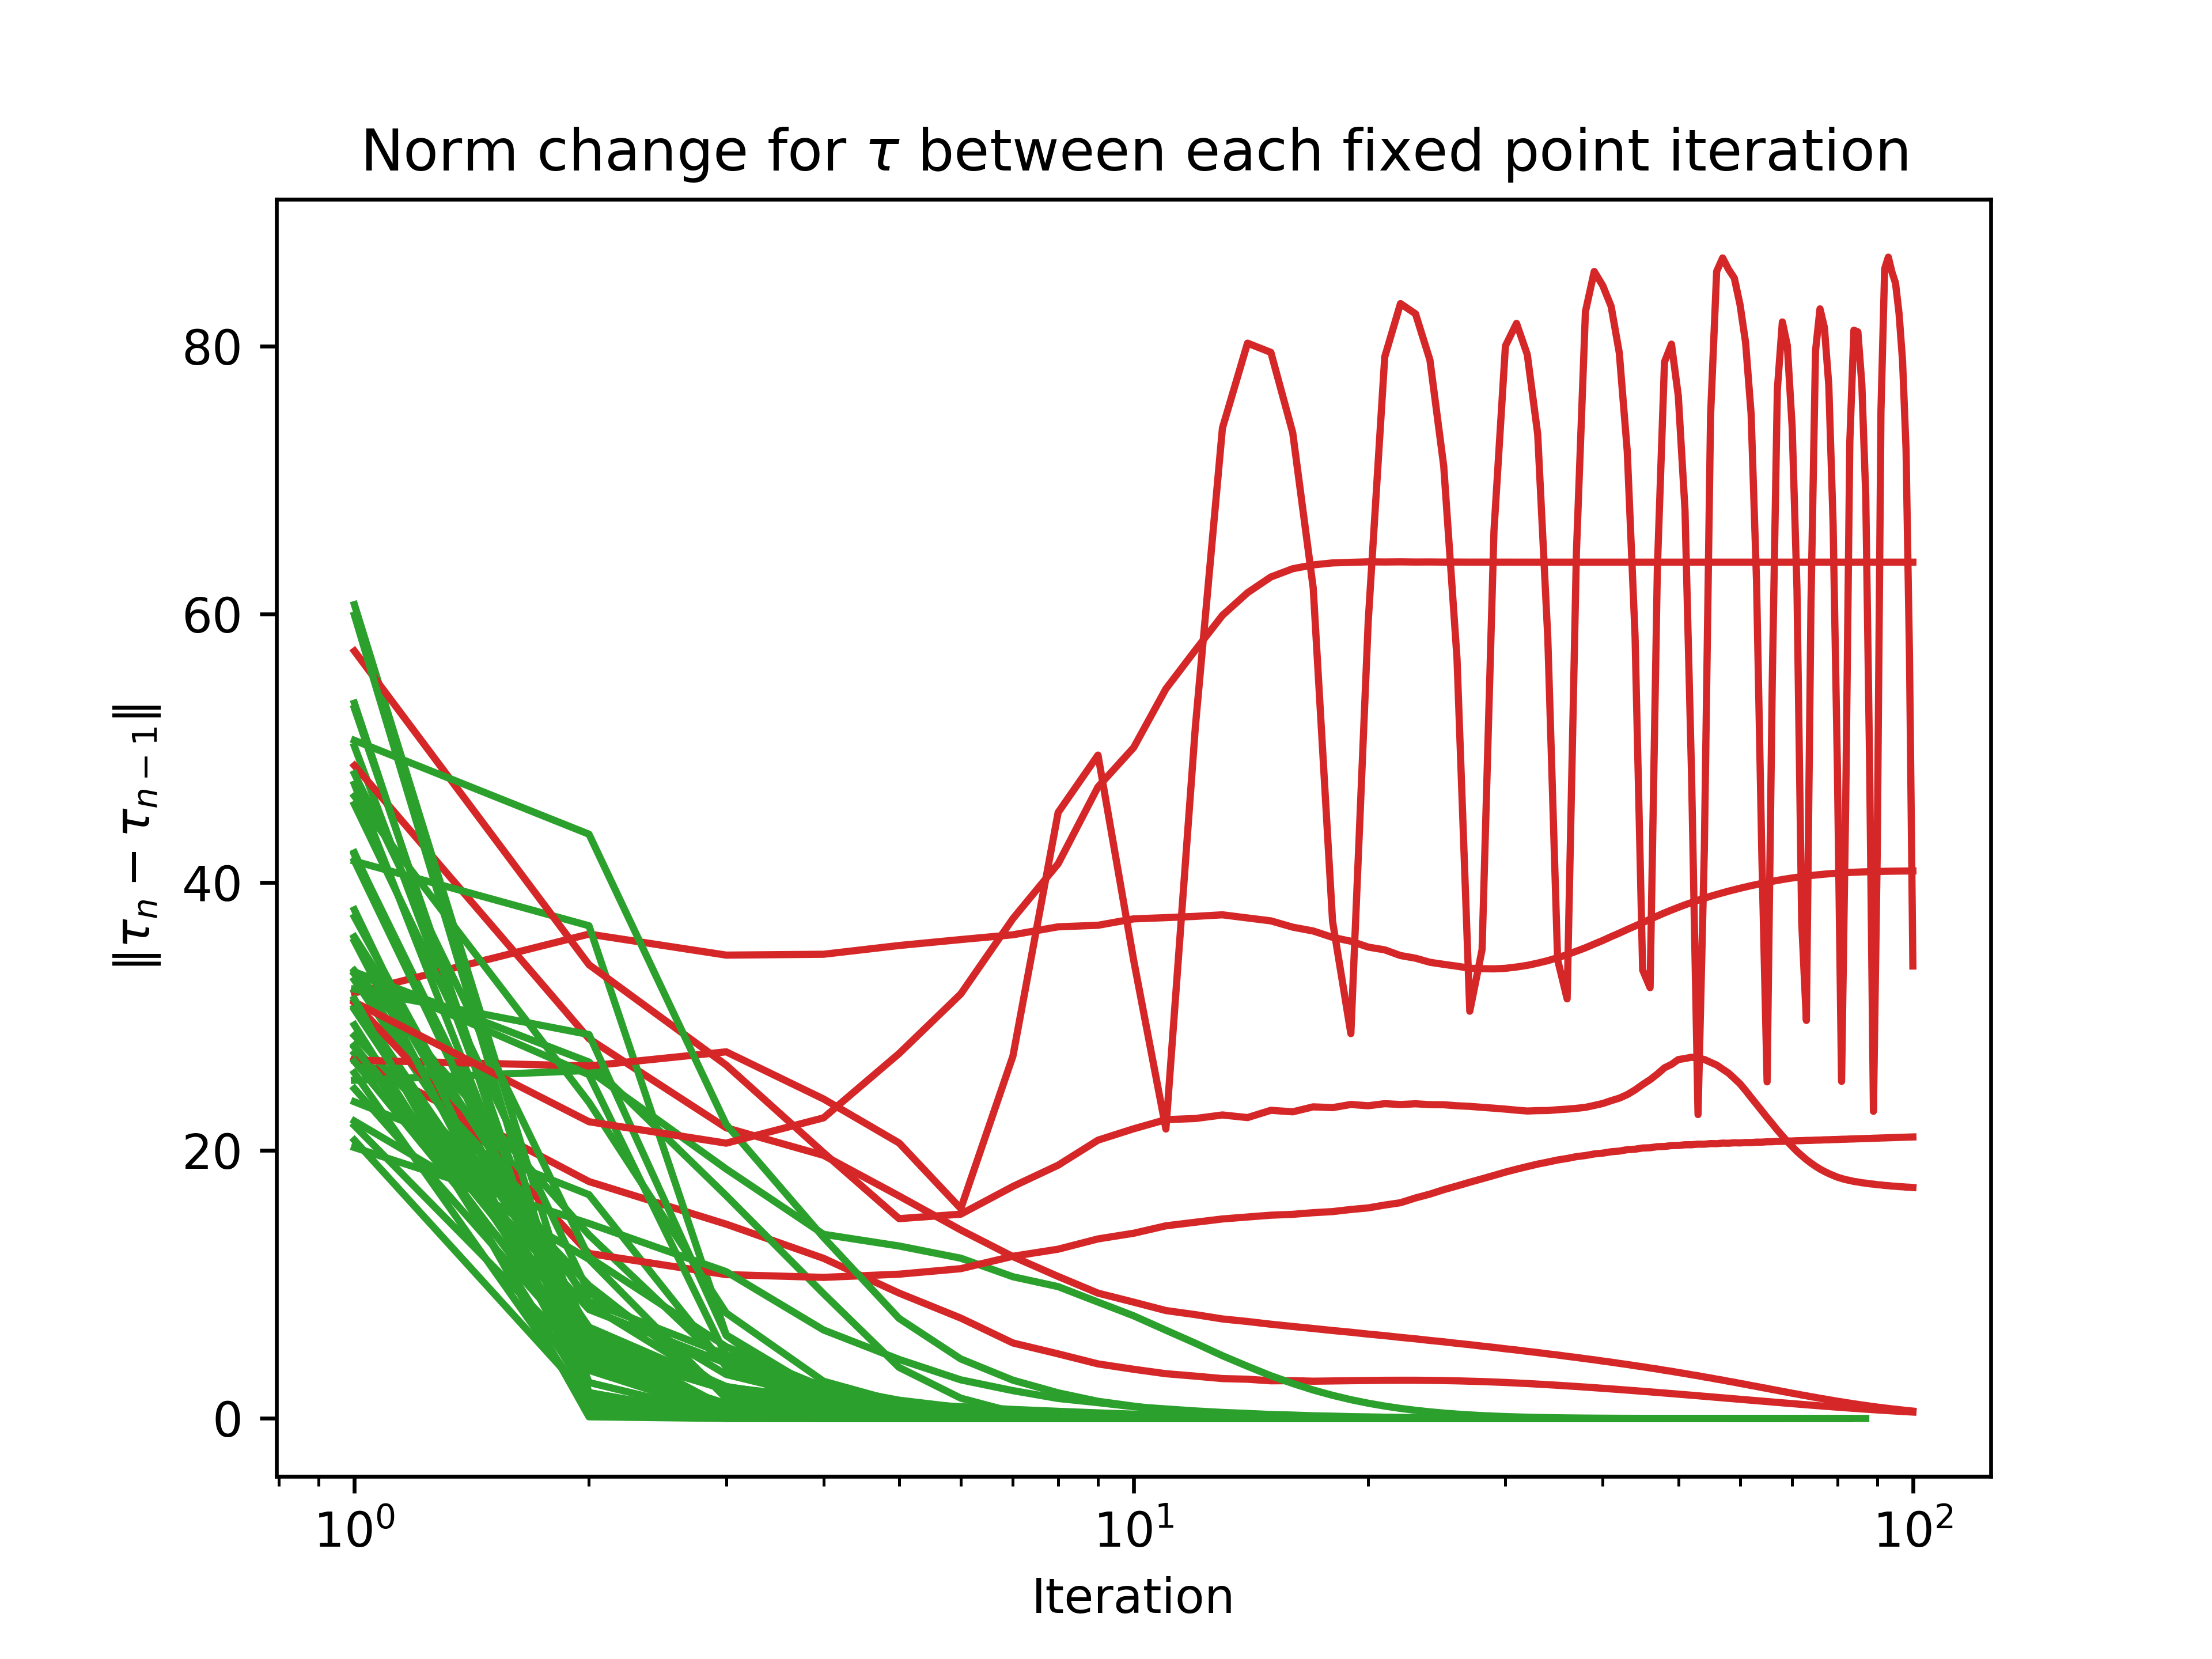
\includegraphics[width=\linewidth]{figures/fixed_point_convergence_fixed_tau.png}
            \caption{Fixed $\tau$, variable $\alpha$, $\pi$ and $\tau$.}
            \label{fig:fixed_point_cv_tau}
        \end{subfigure}
        \begin{subfigure}{0.49\linewidth}
            \centering
            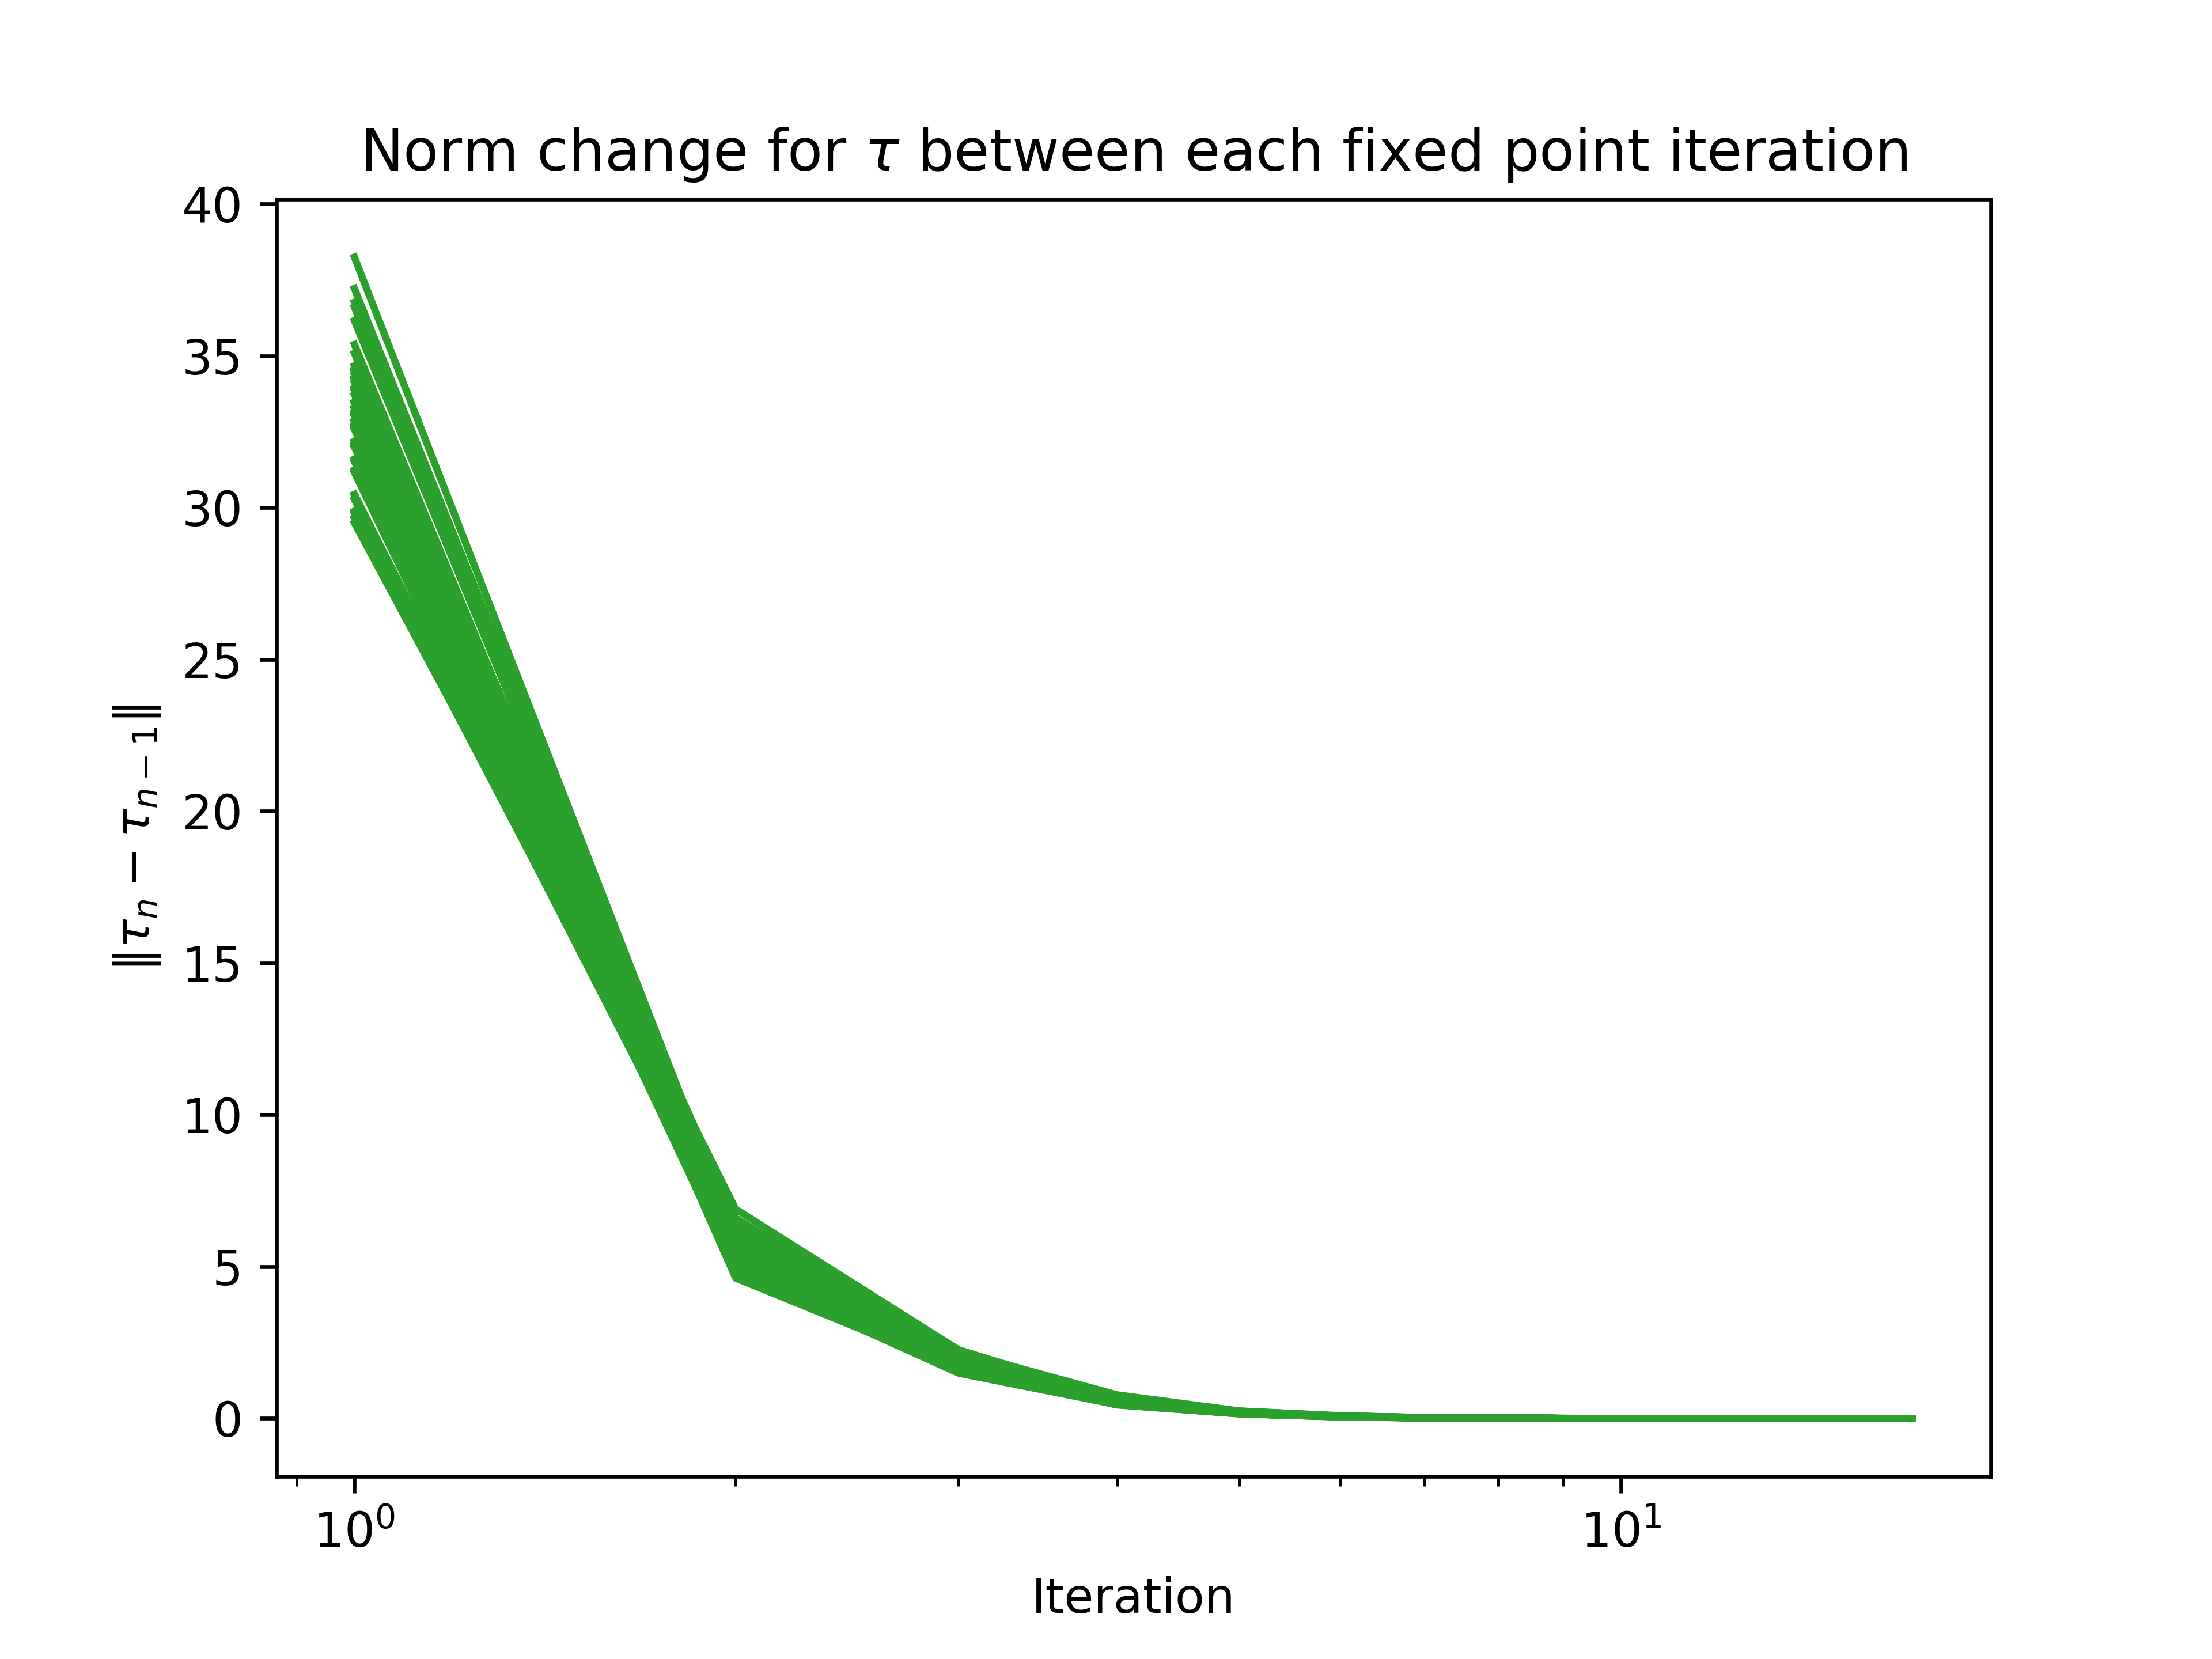
\includegraphics[width=\linewidth]{figures/fixed_point_convergence_fixed_X_alpha_pi.png}
            \caption{Variable $\tau$, fixed $\alpha$, $\pi$ and $\tau$.}
            \label{fig:fixed_point_cv_X}
        \end{subfigure}
        \caption{Convergence of the fixed point algorithm. Green curves converged within $100$ iterations; red curves did not.}
        \label{fig:fixed_point_cv}
    \end{figure*}


    \subsection{Metrics}
    \label{subsec:metrics}

    The literature offers various metrics to assess the quality of a clustering. For our experiments, we re-implemented some supervised and unsupervised metrics.

    \paragraph{Supvervised metrics} By ``supervised metrics'', we designate metrics that compare the labelling of nodes $C^P$ as predicted by a clustering method, with a ground truth labelling $C^T$ that is supposed to be given. We used two classical ones, the Rand index (RI) and the normalized mutal information (NMI).

    RI measures the similarity of two clusterings by measuring how consistently the two clusterings identify edges as connecting nodes of a same cluster, or of different clusters:
    \begin{equation}
        \mathrm{RI} = \frac{a + b}{m}
    \end{equation}
    with $a$ the number of pair of nodes that are in a same clsuter in both clusterings, $b$ the number of pairs of nodes that are in different clusters in both clusterings and $m$ the number of pairs of nodes in the graph.

    MI is a measure that evaluates the mutual dependence between two variables. For two clusters $C = (C_i)_{1 \leq i \leq |C|}$ and $C' = (C'_j)_{1 \leq i \leq |C'|}$, it is defined as
    \begin{equation}
        \mathrm{MI}(C, C') = \sum_{i=1}^{|C|} \sum_{j=1}^{|C'|} P(i, j) \log\left(\frac{P(i,j)}{P(i)P'(j)}\right)
    \end{equation}
    with $P(i) = \frac{|C_i|}{n}$, $P'(j) = \frac{|C'_j|}{n}$ and $P(i,j) = \frac{|C_i \cap C'_j|}{n}$.

    Both measures are insensitive to permutation of the clusters.

    \paragraph{Unsupervised metrics} Unsupervised metrics are defined without resorting to ground truth labelling.

    The modularity M of a clustering is a common metric that compares the observed connectivity within clusters to its expected value for a random graph with the same degree distribution as the considered graph. It is defined as
    \begin{equation}
        \mathrm{M}(C) = \sum_{i=1}^{|C|} \left(\frac{e_i}{m} - \left(\frac{d_i}{2m}\right)^2 \right)
    \end{equation}
    with $m$ the number of edges in the graph, and $e_i$ and $d_i$ respectively the number of edges and total degree of nodes in cluster $C_i$.

    Additionally, we use the clustering coefficient defined as the ratio of all triangles within a set of nodes $C$, over the total number of triplets of nodes within this set; using the adjacency matrix, this writes:
    \begin{equation}
        \mathrm{CC}(C) = \frac{\displaystyle \sum_{i, j, k \in C} X_{ij} X_{jk} X_{ki}}{\displaystyle
            \sum_{i \in C} k_i (k_i - 1)}
    \end{equation}
    with $k_i$ the degree of node $i$. We will use this metric both at the scale of clusters (to determine their individual qualities) and of whole graphs to measure their clustering tendency. To close this section on metrics, note that the SBM model defined in Section \ref{subsec:mixture_model} allows a computation of the expected clustering coefficient associated to graphs generated by a given set of parameters ($\alpha, \pi$):
    \begin{equation}
        \mathrm{CC}_{\mathrm{SBM}} = \frac{\displaystyle  \sum_{q, l, m \in \intset{1}{Q}} \alpha_q \, \alpha_l \, \alpha_m \, \pi_{ql} \, \pi_{qm} \, \pi_{lm}}{\displaystyle  \sum_{q, l, m \in \intset{1}{Q}} \alpha_q \, \alpha_l \, \alpha_m \, \pi_{ql} \, \pi_{qm}}.
    \end{equation}


    \begin{table*}[ht]
        \centering
        \setlength\heavyrulewidth{0.25ex}
        \begin{tabular}{@{}cccccc@{}}
            \toprule
            \multicolumn{2}{c}{\textbf{Experiment}} & \multicolumn{2}{c}{\textbf{Hyper-parameters}} & \multicolumn{2}{c}{\textbf{Parameters}}                                                                                                                                          \\
            \#                                      & Name                                          & $n$                                     & $Q$                    & $\alpha$                                  & $\pi$                                                             \\ \midrule
            1                                       & \multicolumn{1}{c|}{Random-small}             & 30                                      & \multicolumn{1}{c|}{3} & $\alpha \sim \text{Dir}(1.5)$             & $\pi_{ij} \sim \mathcal{U}([0, 1))$                               \\
            2                                       & \multicolumn{1}{c|}{Random-large}             & 500                                     & \multicolumn{1}{c|}{3} & $\alpha \sim \text{Dir}(1.5)$             & $\pi_{ij} \sim \mathcal{U}([0, 1))$                               \\
            3                                       & \multicolumn{1}{c|}{Homophilic}               & 150                                     & \multicolumn{1}{c|}{3} & $\alpha_i = (\frac{1}{Q})_i$              & $\pi_{ii} = 1-\varepsilon_1, \ \pi_{ij} = \varepsilon_2$          \\
            4                                       & \multicolumn{1}{c|}{Homophilic-hard}          & 150                                     & \multicolumn{1}{c|}{5} & $\alpha_i = (\frac{1}{Q})_i$              & $\pi_{ii} \sim \mathcal{U}([0.5, 1)), \ \pi_{ij} = \varepsilon_2$ \\
            5                                       & \multicolumn{1}{c|}{High-degree-minority}     & 150                                     & \multicolumn{1}{c|}{2} & $\alpha^T = (\frac{9}{10}, \frac{1}{10})$ & $\pi = \begin{pmatrix} \varepsilon_2 & a \\ a & b \end{pmatrix}$  \\
            6                                       & \multicolumn{1}{c|}{Heterophilic}             & 150                                     & \multicolumn{1}{c|}{3} & $\alpha_i = (\frac{1}{Q})_i$              & $\pi_{ii} = \varepsilon_2, \ \pi_{ij} = 1 - \varepsilon_1$        \\ \bottomrule
        \end{tabular}
        \caption{Parameters used for the generation of the SBM dataset.}
        \label{tab:sbm_parameters}
    \end{table*}


    \subsection{Testing on SBM datasets}

    This second set of experiments aimed at evaluating the Daudin-EM algorithm is 3-fold:
    \begin{enumerate}
        \item assessing the capacity of the algorithm to recover the parameters of the model that generated a given graph;
        \item assessing the performance of the algorithm in terms of graph clustering;
        \item experimenting with ICL to select the number of clusters. \textcolor{red}{A voir}
    \end{enumerate}


    \paragraph{Bulding the dataset} Using the SBM, we generate 6 batches of $10$ graphs to test the method on. Each batch is generated using a specific set of parameters with the intent of modelling a specific type of graphs, as indicated by the name of the associated experience. The parameters of the SBM for each batch are given in Table \ref{tab:sbm_parameters}, $\mathrm{Dir}$ the Dirichlet law, $\varepsilon_1 = 0.1$, $\varepsilon_2 = 0.01$, $a = 0.7$ and $b = 0.8$. Note that $\pi$ was made symmetric, normalized and scaled in experiments 1 and 2. Sample graphs from each batch are visualized on Figure \ref{fig:sample_graphs} in appendix.

    \paragraph{Assessing parameter recovering performance} Because the graphs are precisely generated using the same model as the one we are trying to fit, these experiments are primarily designed to estimate the performance of the proposed EM algorithm. In particular, a ground truth $(\alpha{\mathrm{T}}, \pi_{\mathrm{T}})$ is trivially given for the expected best-fitting model. Consequently, we could simply measure the distance between the laws induced by the predicted $(\alpha_P, \pi_P)$ and the ground truth $(\alpha{\mathrm{T}}, \pi_{\mathrm{T}})$. However, as explained in \cite{main_article}, the likelihood of an adjacency matrix $X$ given a choice of parameters is intractable, making it hard to apply criteria like the Kullback-Leibler divergence or the $\chi^2$ statistic. We have considered using the relative distance between $\mathcal{J(R_X(\cdot; \tau_P)}$ computed for both sets of parameters, but ditched this metric due to its lack of interpretability across batches. Ultimately, \textcolor{red}{even though this solution is not ideal, [ça vous va ?]} we decided to simply sum the Euclidean distances between $\alpha_T$ and $\alpha_P$ and between $\pi_T$ and $\pi_P$, normalized by the number of classes.

    % Instead, we re-use the lower bound $\mathcal{J}$ introduced in Section \ref{subsec:mixture_model} as a proxy for the likelihood, and compute the relative error $\mathrm{RE}_\J$ between the lower bounds obtained with the ground truth and the predicted parameters. Denoting $(\alpha_P, \pi_P, \tau_P)$ the predicted parameters and $(\alpha_T, \pi_T, z)$ the ground truth used for the generation (with $z$ the value of the latent variable $Z$ sampled from \eqref{eq:prior_Z}), this writes:
    % \begin{equation}
    %     \mathrm{RE}_\J = \frac{\J(R_X(\cdot; \tau_P); \alpha_P, \pi_P) - \J(R_X(\cdot; z); \alpha_T, \pi_T)}{\J(R_X(\cdot; z); \alpha_T, \pi_T)}.
    % \end{equation}
    % Note that taking $R_X(\cdot; z)$ for the ground truth amounts to taking a deterministic law for $Z$, equal to $z$..

    \paragraph{Assessing clustering performance} To assess the clustering capacity of the algorithm, we use the metrics introduced in Section \ref{subsec:metrics}. In particular, the true and predicted clusterings are defined as $\forall i \in \intset{1}{Q}$,
    \begin{equation}
        \quad C^T_i = \argmax_q z_{iq} \quad \text{and} \quad C^P_i = \argmax_q \hat{\tau}_{iq}.
    \end{equation}
    with $\hat{\tau}$ the predicted value of $\tau$ output by the algorithm. For more intepratbility of modularity, instead of averaging over graphs, we choose the graph that produced largest modularity with the predicted parameters.

    \paragraph{Running the experiments} each experiment is run for $100$ iterations, and each time using $5$ random initializations of $\alpha$ and $\pi$ to limit the effects of the lack of robustness underlined in Section \ref{subsec:robustness}.

    The results of the experiments are presented in Table \ref{tab:sbm_results}, along with sample predictions on Figure \ref{fig:pred_graphs} in appendix. Note that, due to the lack of robustness underlined in Section \ref{subsec:robustness}, Daudin-EM did not converge within the budget of $1000$ iterations for all graphs. This is why the number of passed graphs is indicated in the results.


    \subsection{Comparison to variants}

    In the last set of experiments, the Daudin-EM method \cite{main_article} described in Section \ref{subsec:mixture_model} is tested on real graphs and compared with 2 other methods:
    \begin{enumerate}
        \item The alternative mixture model from \cite{newman} described in section \ref{subsec:newman};
        \item The spectral clustering method from \cite{spectral} described in section \ref{subsec:spectral}.
    \end{enumerate}

    The results are then visualized and compared in terms of running time and clustering power, using the metrics defined in Section \ref{subsec:metrics}.
    \paragraph{Datasets}
    These methods are all tested on 2 famous datasets, commonly used as benchmarks for community detection algorithms:
    \begin{enumerate}
        \item Zachary's Karate-club dataset: Published in an Anthropology journal in 1977 \cite{karate}, it describes the friendship between 34 members of a karate club at a US university after an internal dispute that split the social relationships in two factions. The graph is undirected and contains 34 nodes and 78 edges. Figure \ref{fig:zachary_gt} shows the ground truth of the dataset.
        \item The Cora dataset: A citation network of scientific publications \cite{cora}. The graph is undirected and contains 2708 nodes(=papers) and 5429 edges(=citations). The nodes are labeled with 7 different classes. Figure \ref{fig:cora_gt} shows the dot-plot representation of the adjacency matrix of the ground truth, with associated labels.
    \end{enumerate}
    While the Karate-club dataset is a small graph with a clear community structure, the Cora dataset is a much larger graph with a more complex structure. Both datasets are constructed from real-world data and observations which makes them interpretable. They also have a ground truth that we can use to evaluate the performance of the algorithms.

    \paragraph{Running the experiments} For Zachary's karate club, Daudin-EM and Newman-EM are run for $100$ iterations. For Daudin-EM, using $20$ parallel initializations of $(\alpha, \pi, \tau)$ to increase probability of converging.
    For Cora, they are run for $50$ iterations, using $10$ initializations of $(\alpha, \pi, \tau)$.
    In both cases, the spectral clustering algorithm is run once.

    Figures \ref{fig:zachary_results} and \ref{fig:cora_results} show for both datasets the true clusterings and those proposed by the 3 methods, and tables \ref{tab:zachary_results} and \ref{tab:cora_results} show the resulting metrics.






    \section{Results discussion}
    \label{sec:discussion}

    \paragraph{First set of experiments}
    From the first set of experiments, we understand that the main weakness of Daudin-EM is the difficult convergence of the fixed-point algorithm of the E-step. In particular, as observed on Figure \ref{fig:fixed_point_cv}, this algorithm is particularly sensitive to the initialization on $(\alpha, \pi)$, but not as much on the initialization of $\tau$. Some ideas have been tested to solve this, such as applying a momentum-based formula of the form $\hat{\tau}_{n+1} = \hat{\tau}_{n} + \gamma \hat{\tau}_{n}^{\mathrm{FP}}$ for the $n$\textsuperscript{th} E-step, with $\gamma$ an update rate and $\hat{\tau}_{n}^{\mathrm{FP}}$ the result of the fixed-point algorithm; but this showed little improvement.

    \paragraph{Second set of experiments}
    In the SBM experiments, we observe that Daudin-EM performs generally rather poorly, both for fitting the SBM and clustering graphs. In particular, it has a tendency to predict only one cluster (resulting in null NMI), especially for clear-cut clusters (both homophilic and heterophilic). On the other hand, it brings better model-fitting performance for random graphs, especially large ones, and also yields high supervised metrics in this case. Lastly, it achieves near-perfect results for the ``High-degree-minority'' case of experiment 5 according to both criteria, with a modularity that is rightly negative in this instance of graph type.

    To sum up, Daudin-EM seems bad at detecting clusters, especially rather homogeneous ones. Our main observation is that this method seems very sensitive to the distribution of degrees of nodes, as rather homogeneous clusters are hardly distinguished by this quantity. This would also explain the best results observed for experiment 5. One way to alleviate this problem might be to offer semi-supervised guidance to enforce a favourable initialization.

    \paragraph{Third set of experiments} For both datasets, Daudin-EM brings mostly dissatisfying performance, especially when compared with Newman which always give the best results. As for the spectral clustering method, it is behaves well on Zachary's karate club, but very badly on Cora, probably due to its large size. Daudin-EM is also particularly slow, notably due to the number of iterations required for convergence of the E-step.

    For Zachary's karate club, Daudin-EM yields low NMI and RI, as well as a negative modularity. On the other hand, the resulting per-cluster clustering coefficients are higher than that of the ground truth clusters in average, thus revealing clusters of better quality from that perspective.

    On the other hand, Daudin-EM brought interesting results for Cora. Indeed, the supervised metrics are comparable to those for Newman-EM. Furthermore, although the final modularity is quite low with Daudin-EM, and despite some clusters having a clustering coefficient of 0, the method reveals some good-quality clusters, especially clusters 2 and 4. Additionally, cluster 5 is interesting as it gathers papers that cite (or are cited by) many papers from many different themes, as is probably the case for papers that fall within the ``neural networks'' category. Thereby, the method succeeds to bring a new perspective to the dataset that does not restrict to homophily-driven clustering.


    \section{Conclusion}
    \label{sec:conclusion}

    The SBM-based variational EM method introduced by Daudin \textit{et. al.} in \cite{main_article} has been presented, along with another EM-method from Newman \& Leicht \cite{newman} and the spectral-clustering baseline. Daudin-EM relies on an approximate maximization of the log-likelihood of the law induced by the SBM model, to circumvent the intractability of this law and of its conditional law given the membership of nodes to classes. We have illustrated that the main flaw of this algorithm is the unproven and unreliable convergence of the fixed-point-based E-step, a flaw not shared by Newman-EM which benefits from a closed-form solution. This is at the root of a lack of robustness of the method as well as to its lengthy execution due to numerous iterations. Testing on several datasets revealed poor performance of the method against Newman-EM, but better performance against spectral clustering on Cora. In particular, the experiments hinted towards a large sensitivity of the method node degree distributions and a tendency to gather nodeds into clusters as large as possible. [better perf on large graphs and reveals properties different from other clustering methods]


    \newpage

    \bibliography{bibliography}

\end{multicols}

\newpage


\appendix

\begin{center}
    {\Huge \bfseries Appendix} \\[0.5cm]
\end{center}

\section{Implementations speed comparison}
\label{app:speed_comparison}

\begin{figure}[h]
    \centering
    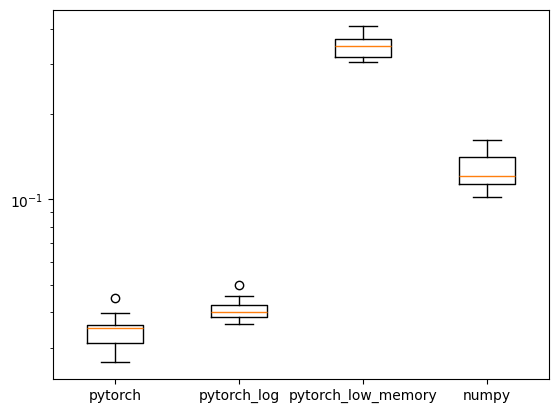
\includegraphics[width=0.5\linewidth]{figures/speed_comparison_VEM.png}
    \caption{Speed comparison (in seconds) between implementations of the SBM-VEM for the mixture model. Each implementation was run 10 times, for 10 runs on a graph randomly generated using SBM for 100 nodes and 3 classes.}
    \label{fig:speed_comparison}
\end{figure}

\newpage

\section{Second set of experiments}
\label{app:sbm}

\subsection{Samples}

\hphantom{.}  % Force figure to go here

\begin{figure*}[h]
    \hfill
    \centering
    \begin{subfigure}{0.28\linewidth}
        \centering
        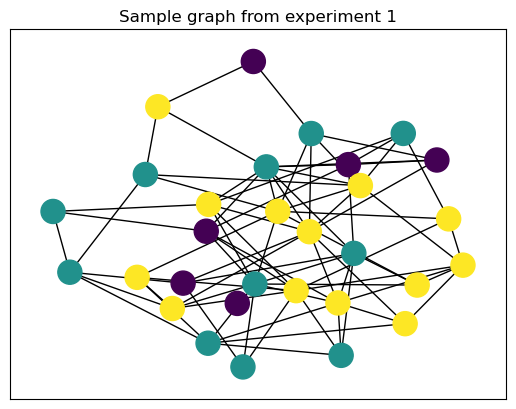
\includegraphics[width=\linewidth]{figures/exp1_sample.png}
    \end{subfigure}
    \hfill
    \begin{subfigure}{0.28\linewidth}
        \centering
        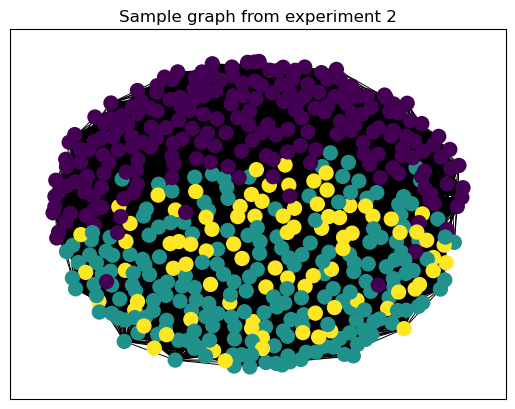
\includegraphics[width=\linewidth]{figures/exp2_sample.png}
    \end{subfigure}
    \hfill
    \begin{subfigure}{0.28\linewidth}
        \centering
        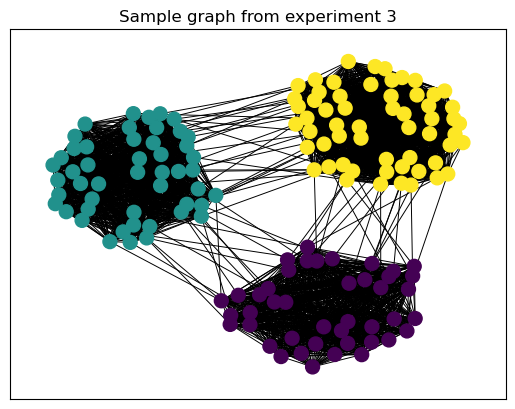
\includegraphics[width=\linewidth]{figures/exp3_sample.png}
    \end{subfigure}
    \hfill

    \medskip

    \hfill
    \begin{subfigure}{0.28\linewidth}
        \centering
        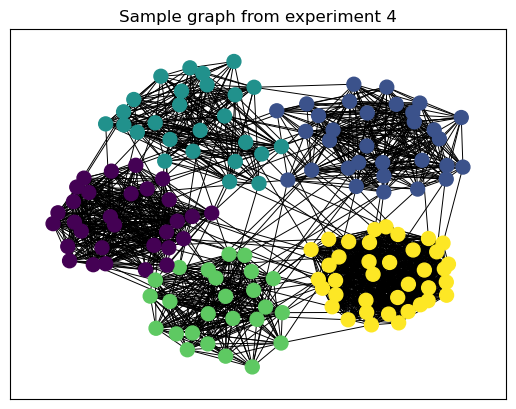
\includegraphics[width=\linewidth]{figures/exp4_sample.png}
    \end{subfigure}
    \hfill
    \begin{subfigure}{0.28\linewidth}
        \centering
        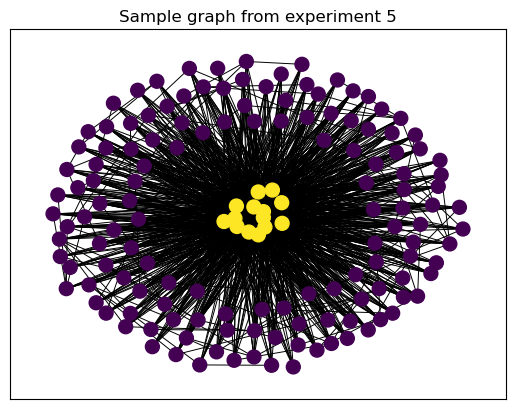
\includegraphics[width=\linewidth]{figures/exp5_sample.png}
    \end{subfigure}
    \hfill
    \begin{subfigure}{0.28\linewidth}
        \centering
        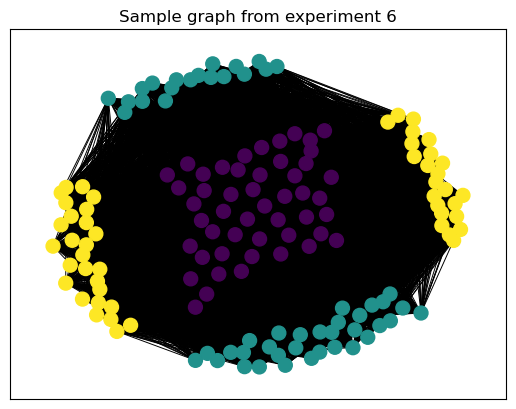
\includegraphics[width=\linewidth]{figures/exp6_sample.png}
    \end{subfigure}
    \hfill
    \caption{Sample graphs from the second set of experiments}
    \label{fig:sample_graphs}
\end{figure*}

\subsection{Results}

\hphantom{.}

\begin{figure*}[h]
    \hfill
    \centering
    \begin{subfigure}{0.28\linewidth}
        \centering
        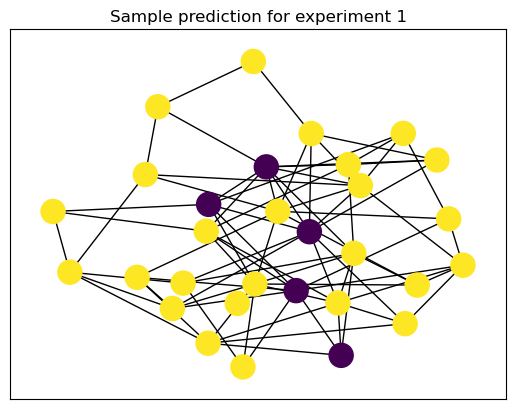
\includegraphics[width=\linewidth]{figures/exp1_pred.png}
    \end{subfigure}
    \hfill
    \begin{subfigure}{0.28\linewidth}
        \centering
        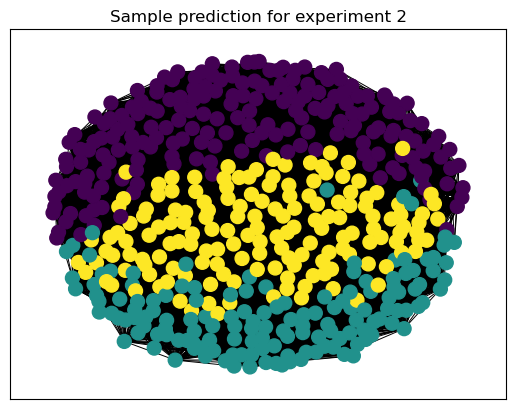
\includegraphics[width=\linewidth]{figures/exp2_pred.png}
    \end{subfigure}
    \hfill
    \begin{subfigure}{0.28\linewidth}
        \centering
        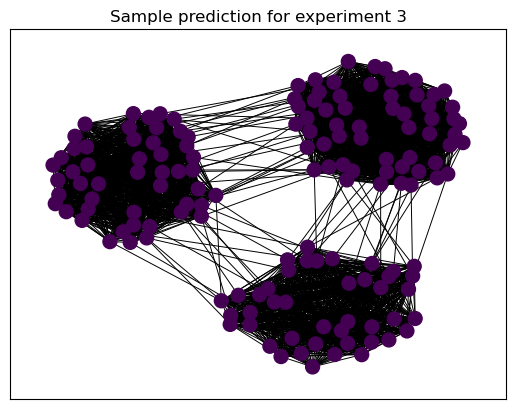
\includegraphics[width=\linewidth]{figures/exp3_pred.png}
    \end{subfigure}
    \hfill

    \medskip

    \hfill
    \begin{subfigure}{0.28\linewidth}
        \centering
        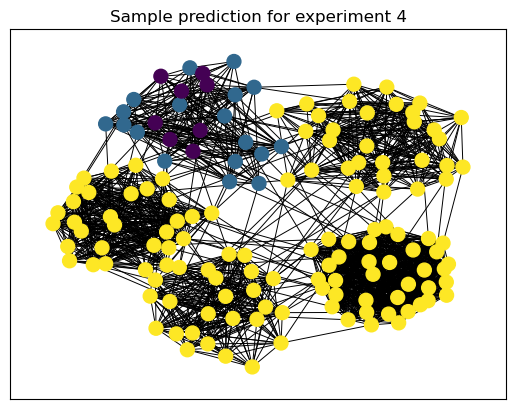
\includegraphics[width=\linewidth]{figures/exp4_pred.png}
    \end{subfigure}
    \hfill
    \begin{subfigure}{0.28\linewidth}
        \centering
        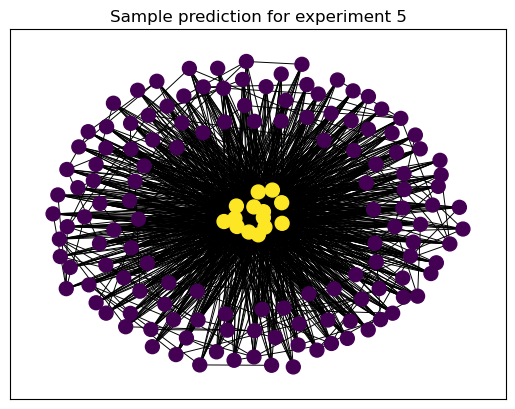
\includegraphics[width=\linewidth]{figures/exp5_pred.png}
    \end{subfigure}
    \hfill
    \begin{subfigure}{0.28\linewidth}
        \centering
        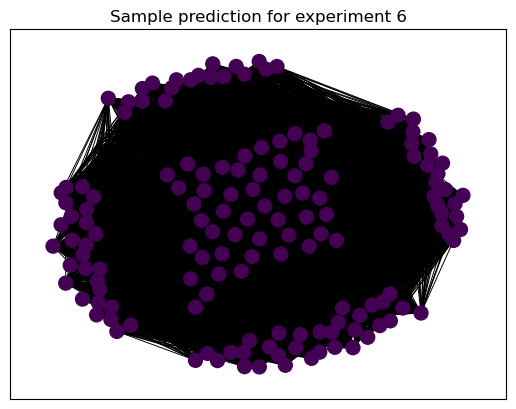
\includegraphics[width=\linewidth]{figures/exp6_pred.png}
    \end{subfigure}
    \hfill
    \caption{Some predicted graphs from the second set of experiments}
    \label{fig:pred_graphs}
\end{figure*}

\begin{table*}[h]
    \centering
    \setlength\heavyrulewidth{0.25ex}
    \begin{tabular}{@{}ccccccc@{}}
        \toprule
        Experiment \# & \# graphs passed        & Param. dist.                         & NMI             & RI               & G.t. M & Pred. M \\ \midrule
        1             & \multicolumn{1}{c|}{10} & \multicolumn{1}{c|}{$0.13 \pm 0.06$} & $0.07 \pm 0.07$ & $0.52 \pm  0.10$ & 0.08   & 0.02    \\
        2             & \multicolumn{1}{c|}{8}  & \multicolumn{1}{c|}{$0.08 \pm 0.03$} & $0.33 \pm 0.13$ & $0.66 \pm 0.13$  & 0.07   & 0.07    \\
        3             & \multicolumn{1}{c|}{10} & \multicolumn{1}{c|}{$0.22 \pm 0.12$} & $0 \pm 0$       & $0.33 \pm 0.00$  & 0.63   & 0.00    \\
        4             & \multicolumn{1}{c|}{4}  & \multicolumn{1}{c|}{$0.22 \pm 0.02$} & $0.11 \pm 0.18$ & $0.27 \pm 0.12$  & 0.71   & 0.15    \\
        5             & \multicolumn{1}{c|}{10} & \multicolumn{1}{c|}{$0.02 \pm 0.01$} & $1 \pm 0$       & $1 \pm 0$        & -0.38  & -0.38   \\
        6             & \multicolumn{1}{c|}{9}  & \multicolumn{1}{c|}{$0.18 \pm 0.08$} & $0 \pm 0$       & $0.33 \pm 0.00$  & -0.33  & 0.00    \\ \bottomrule
    \end{tabular}
    \caption{Results of the second set of experiments.}
    \label{tab:sbm_results}
\end{table*}

\newpage

\section{Third set of experiments}
\label{app:real}

\subsection{Zachary's Karate club}
\label{app:zachary}

\hphantom{.}

\begin{figure*}[h]
    \centering
    \begin{subfigure}{0.42\linewidth}
        \centering
        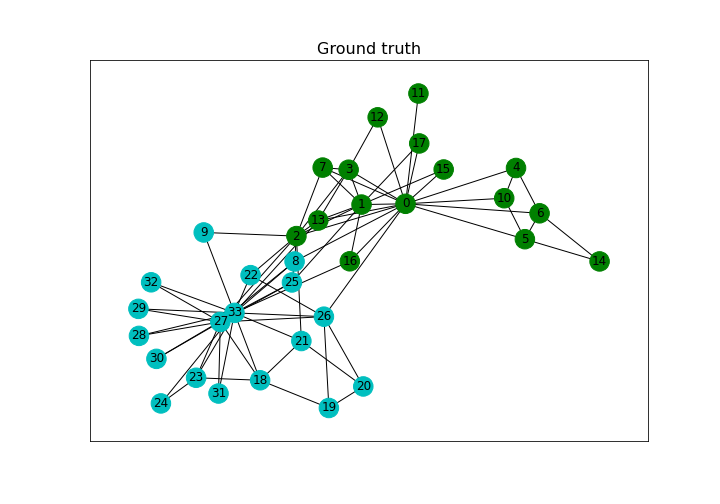
\includegraphics[width=\linewidth, trim={45 35 35 60}, clip]{figures/karate_club_gt.png}
        \caption{Ground truth.}
        \label{fig:zachary_gt}
    \end{subfigure}
    \hspace{1em}
    \begin{subfigure}{0.42\linewidth}
        \centering
        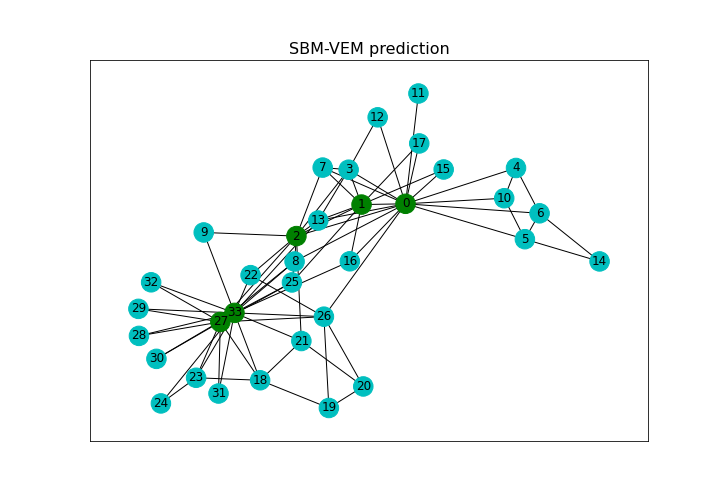
\includegraphics[width=\linewidth, trim={45 35 35 60}, clip]{figures/karate_club_sbm.png}
        \caption{Clustering proposed by the SBM-VEM method.}
        \label{fig:zachary_SBM}
    \end{subfigure}

    \medskip

    \begin{subfigure}{0.42\linewidth}
        \centering
        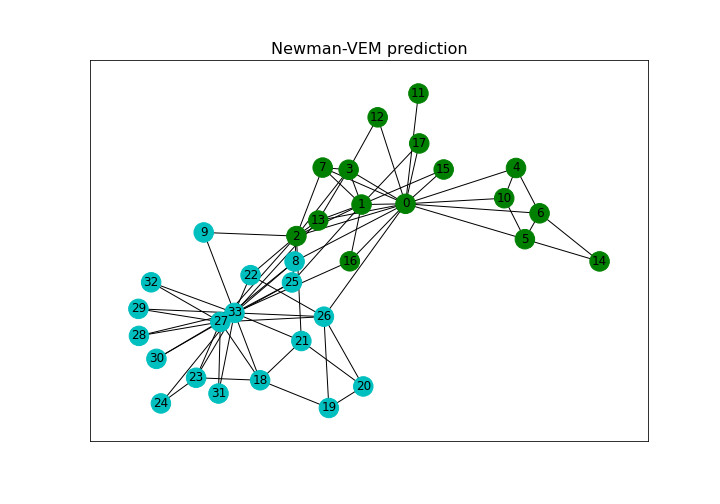
\includegraphics[width=\linewidth, trim={45 35 35 60}, clip]{figures/karate_club_newman.png}
        \caption{Clustering proposed by the Newman SBM method.}
        \label{fig:zachary_newman}
    \end{subfigure}
    \hspace{1em}
    \begin{subfigure}{0.42\linewidth}
        \centering
        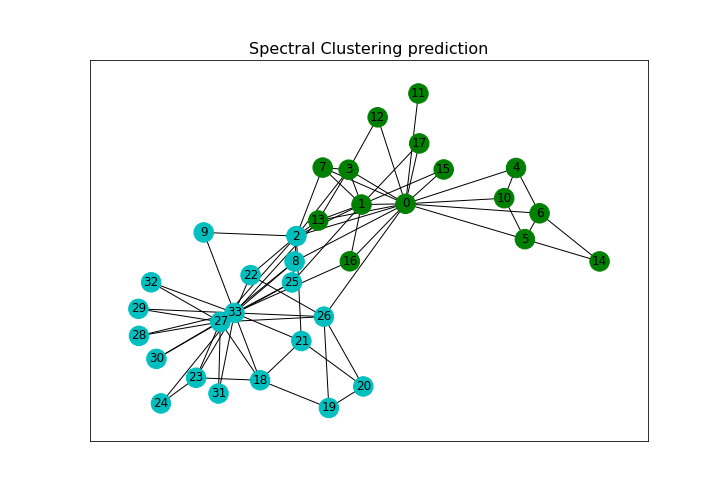
\includegraphics[width=\linewidth, trim={45 35 35 60}, clip]{figures/karate_club_spectral.png}
        \caption{Clustering proposed by the spectral method.}
        \label{fig:zachary_spectral}
    \end{subfigure}
    \caption{Clustering results for Karate Club.}
    \label{fig:zachary_results}
\end{figure*}

\begin{table*}[h]
    \centering
    \setlength\heavyrulewidth{0.25ex}
    \begin{tabular}{@{}cccccccc@{}}
        \toprule
        \multirow{2}{*}{\textbf{Method}}  & \multirow{2}{*}{\textbf{Time (s)}} & \multirow{2}{*}{\textbf{NMI}} & \multirow{2}{*}{\textbf{RI}} & \multirow{2}{*}{\textbf{M}} & \multirow{2}{*}{\textbf{CC}} & \multicolumn{2}{c}{\textbf{CC (per cluster)}}        \\
                                          &                                    &                               &                              &                             &                              & 1                                             & 2    \\ \midrule
        \multicolumn{1}{c|}{Ground truth} & \multicolumn{1}{c|}{-}             & -                             & \multicolumn{1}{c|}{-}       & 0.37                        & 0.26                         & 0.42                                          & 0.26 \\
        \multicolumn{1}{c|}{Daudin-EM}    & \multicolumn{1}{c|}{137}           & 0.01                          & \multicolumn{1}{c|}{0.49}    & -0.21                       & -                            & 0.50                                          & 0.23 \\
        \multicolumn{1}{c|}{Newman-EM}    & \multicolumn{1}{c|}{2}             & 1.00                          & \multicolumn{1}{c|}{1.00}    & 0.37                        & -                            & 0.41                                          & 0.26 \\
        \multicolumn{1}{c|}{Spectral}     & \multicolumn{1}{c|}{0}             & 0.84                          & \multicolumn{1}{c|}{0.94}    & 0.36                        & -                            & 0.35                                          & 0.24 \\ \bottomrule
    \end{tabular}
    \caption{Results on Zachary’s Karate Club}
    \label{tab:zachary_results}
\end{table*}

\newpage

\subsection{Cora}
\label{app:cora}

\hphantom{.}

\begin{figure}[H]
    \centering
    \hfill
    \begin{subfigure}{0.45\linewidth}
        \centering
        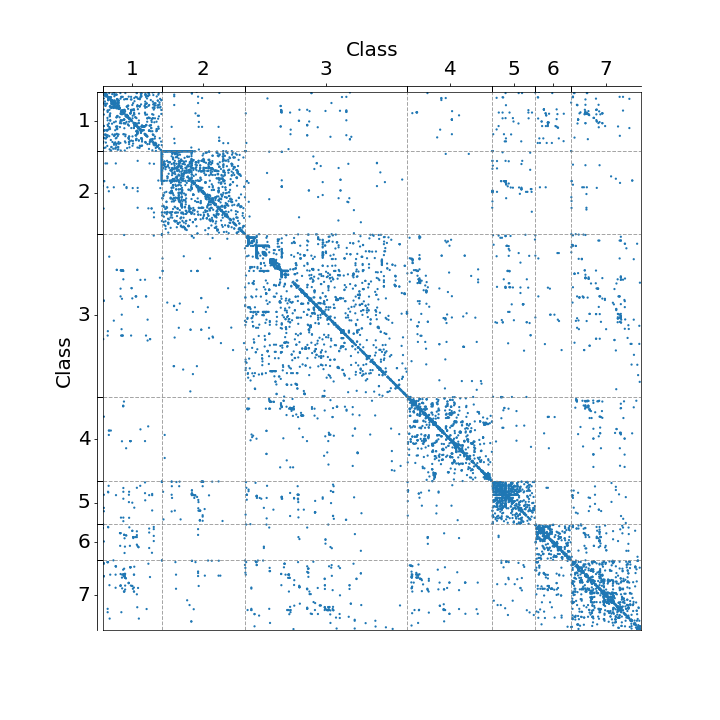
\includegraphics[width=\linewidth, trim={45 35 35 40}, clip]{figures/cora_gt.png}
        \caption{Ground truth.}
        \label{fig:cora_gt}
    \end{subfigure}
    \hfill
    \begin{subfigure}{0.45\linewidth}
        \centering
        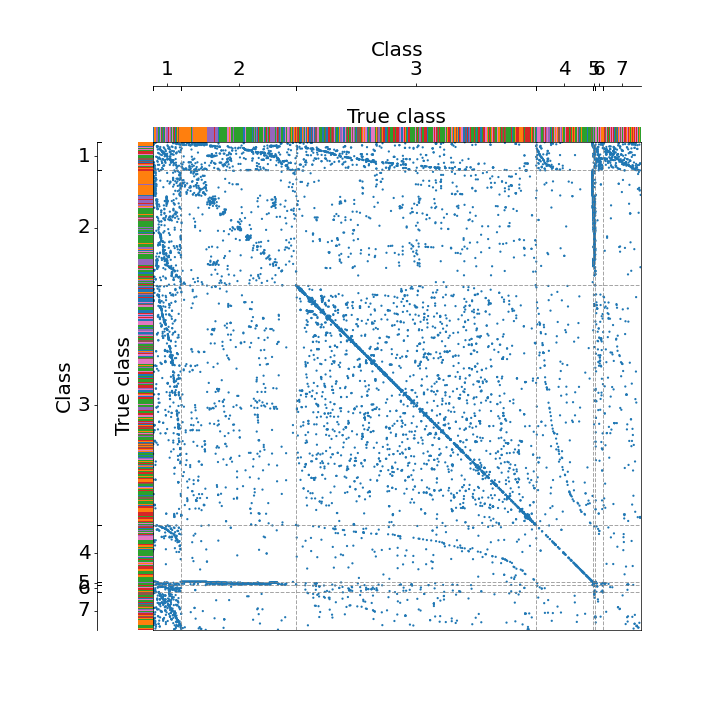
\includegraphics[width=\linewidth, trim={45 35 35 40}, clip]{figures/cora_SBM.png}
        \caption{Clustering proposed by Daudin-EM.}
        \label{fig:cora_SBM}
    \end{subfigure}
    \hfill

    \medskip

    \hfill
    \begin{subfigure}{0.45\linewidth}
        \centering
        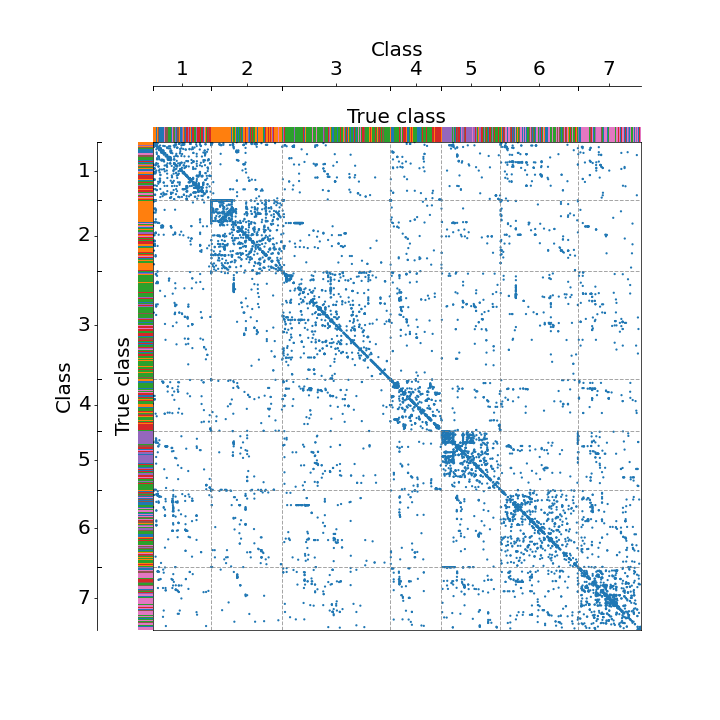
\includegraphics[width=\linewidth, trim={45 35 35 40}, clip]{figures/cora_Newman.png}
        \caption{Clustering proposed by Newman-EM method.}
        \label{fig:cora_newman}
    \end{subfigure}
    \hfill
    \begin{subfigure}{0.45\linewidth}
        \centering
        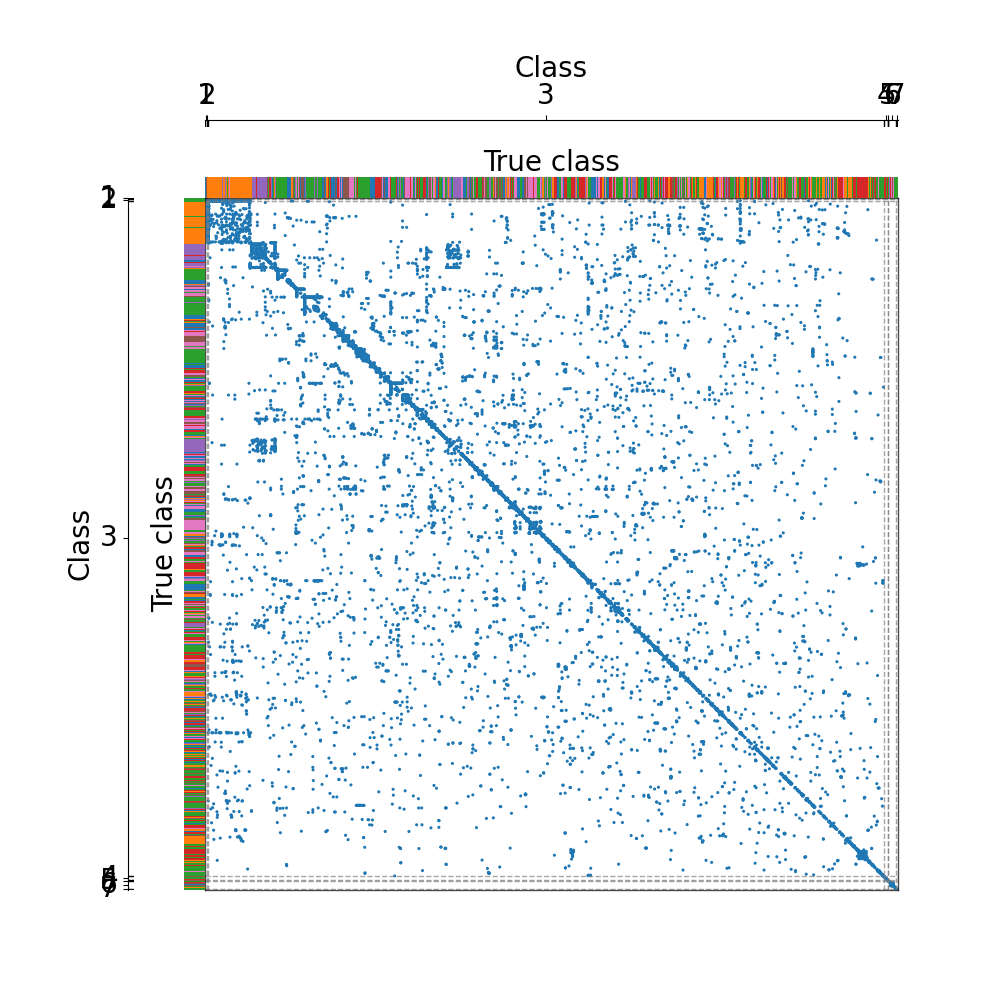
\includegraphics[width=\linewidth, trim={35 25 25 30}, clip]{figures/cora_spetral.png}
        \caption{Clustering proposed by the spectral method.}
        \label{fig:cora_spectral}
    \end{subfigure}
    \hfill
    \caption{Dot-plot of the results for Cora.}
    \scriptsize{G.T.: 1: Case Based; 2: Genetic Algorithms; 3: Neural Networks; 4: Probabilistic Methods; 5: Reinforcement Learning; 6: Rule Learning; 7: Theory.}
    \label{fig:cora_results}
\end{figure}

\begin{table}[H]
    \centering
    \setlength\heavyrulewidth{0.25ex}
    \begin{tabular}{@{}ccccccccccccc@{}}
        \toprule
        \multirow{2}{*}{\textbf{Method}}  & \multirow{2}{*}{\textbf{Time (s)}} & \multirow{2}{*}{\textbf{NMI}} & \multirow{2}{*}{\textbf{RI}} & \multirow{2}{*}{\textbf{M}} & \multirow{2}{*}{\textbf{CC}} & \multicolumn{7}{c}{\textbf{CC (per cluster)}}                                           \\
                                          &                                    &                               &                              &                             &                              & 1                                             & 2    & 3    & 4    & 5    & 6    & 7    \\ \midrule
        \multicolumn{1}{c|}{Ground truth} & \multicolumn{1}{c|}{-}             & -                             & \multicolumn{1}{c|}{-}       & 0.64                        & 0.09                         & 0.19                                          & 0.06 & 0.12 & 0.23 & 0.10 & 0.22 & 0.16 \\
        \multicolumn{1}{c|}{Duadin-EM}    & \multicolumn{1}{c|}{3802}          & 0.15                          & \multicolumn{1}{c|}{0.70}    & 0.22                        & -                            & 0                                             & 0.16 & 0    & 0.29 & 0.25 & 0    & 0.86 \\
        \multicolumn{1}{c|}{Newman-EM}    & \multicolumn{1}{c|}{27}            & 0.18                          & \multicolumn{1}{c|}{0.76}    & 0.53                        & -                            & 0.25                                          & 0.06 & 0.16 & 0.28 & 0.12 & 0.29 & 0.18 \\
        \multicolumn{1}{c|}{Spectral}     & \multicolumn{1}{c|}{1}             & 0.02                          & \multicolumn{1}{c|}{0.23}    & 0.03                        & -                            & 0.6                                           & 0.09 & 0    & 0    & 0    & 0    & 0    \\ \bottomrule
    \end{tabular}
    \caption{Results on Cora.}
    \label{tab:cora_results}
\end{table}


\end{document}